%\setcounter{chapter}{32}

\chapter{Training for Robustness and Generality}
\label{chapter:data_augmentation}

\section{Introduction}

In the previous chapter, we saw that performance of a vision system can look quite good on a training set but fail dramatically when deployed in the real world, and the reason is often distribution shift. How can we train models that are more robust to these kinds of shifts?

This chapter presents several strategies that all have the same goal: broaden the training distribution so that the test data just looks like more of the training data. The following sections present two ways of doing this.

\section{Data Augmentation}

\index{Data augmentation}{\bf Data augmentation} augments a dataset by adding random transformations of each datapoint. For example, below we show some common data augmentations applied to an example image (\fig{\ref{fig:data_augmentation:data_aug_examples}}):
\vspace{-0.5cm}
\begin{figure}[h]
\centerline{
\begin{tikzpicture}%[>=spaced latex]
\def\imgwidth{.13\textwidth}
\def\labelheight{0.08\textwidth}
\def\imgstep{1.15*\imgwidth}
\node at (0,\labelheight) {Original}; \node at (1.5*\imgstep,\labelheight) {\small \texttt{mirror}}; \node at (3.4*\imgstep,4+\labelheight) {$\overbrace{\quad\quad\quad\quad\quad\quad\quad\quad\quad\quad\quad\quad\quad\quad\quad}^{\text{{\small \texttt{crops}}}}$}; \node at (5.3*\imgstep,\labelheight*1.35) {\small \texttt{color}}; \node at (5.3*\imgstep,\labelheight) {\small \texttt{jitter}};
\node[inner sep=0pt] at (0,0)
    {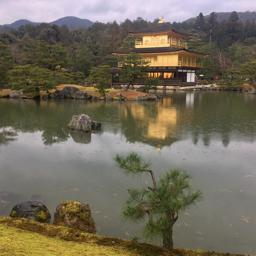
\includegraphics[width=\imgwidth]{./figures/data_augmentation/data_aug_example_original.jpg}};
\draw[thick] [flow_arrow] (6+0.5*\imgwidth,0) -- (0.5*\imgwidth+0.5*\imgstep,0);
\node[inner sep=0pt] at (1.5*\imgstep,0)
    {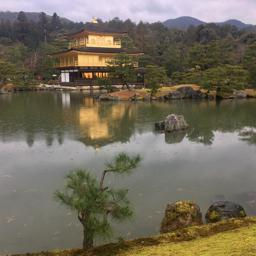
\includegraphics[width=\imgwidth]{./figures/data_augmentation/data_aug_example_mirror.jpg}};
\node[inner sep=0pt] at (2.5*\imgstep,0)
    {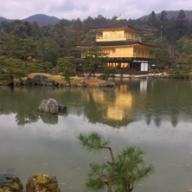
\includegraphics[width=\imgwidth]{./figures/data_augmentation/data_aug_example_crop1.jpg}};
\node[inner sep=0pt] at (3.4*\imgstep,0)
    {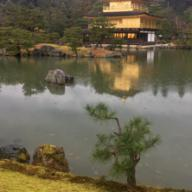
\includegraphics[width=\imgwidth]{./figures/data_augmentation/data_aug_example_crop2.jpg}};
\node[inner sep=0pt] at (4.3*\imgstep,0)
    {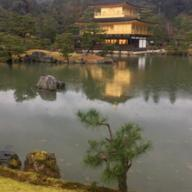
\includegraphics[width=\imgwidth]{./figures/data_augmentation/data_aug_example_crop3.jpg}};
\node[inner sep=0pt] at (5.3*\imgstep,0)
    {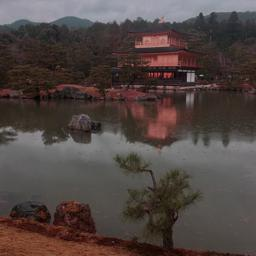
\includegraphics[width=\imgwidth]{./figures/data_augmentation/data_aug_example_color_jitter.jpg}};
\end{tikzpicture}
}
\caption{A few common types of data augmentation.}
\label{fig:data_augmentation:data_aug_examples}
\end{figure}
\marginnote{Data augmentation might not seem not seem very glamorous, but it is one of the most important tools at our disposal. Machine learning is data-driven intelligence, and the bigger the data the better. Data augmentation is like a philosopher's stone of machine learning: it converts lead (small data) into gold (big data).}[2.0cm]

When you do this for every image in a dataset, you are essentially mapping from a smaller dataset to a larger dataset. We know that more data is usually better, so this is a way to simulate the effect of adding more real data to your dataset.
\begin{center}
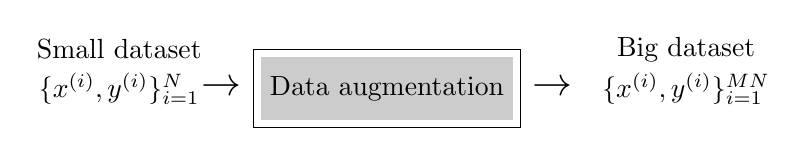
\begin{tikzpicture}
    \draw (0,0) rectangle (3.4,1); % outer box
    \fill[black!20] (0.1,0.1) rectangle (3.3,0.9); % gray box
    \node[] at (1.7,0.5) {Data augmentation};
    \node[] at (-1.7,1) {Small dataset};
    \node[] at (-1.7,0.5) {$\{x^{(i)}, y^{(i)}\}_{i=1}^N$};
    \node[] at (-0.4,0.5) {{\Large  $ \rightarrow$}};
    \node[] at (5.5,1) {Big dataset};
    \node[] at (5.5,0.5) {$\{x^{(i)}, y^{(i)}\}_{i=1}^{MN}$};
    \node[] at (3.8,0.5) {{\Large  $ \rightarrow$}};
\end{tikzpicture}
\end{center}

The way data augmentation works is that for each $\{\mathbf{x}^{(i)}, \mathbf{y}^{(i)}\}$ pair in your original dataset, you add $M$ new synthetic pairs $\{T(\mathbf{x}^{(i)};\theta^{(j)}), \mathbf{y}^{(i)}\}_{j=1}^M$, where $T$ is a data transformation function with stochastic parameters $\theta \sim p_{\theta}$. As an example, $T$ might be the \texttt{crop} function, and then $\theta$ would be a set of coordinates specifying where to apply the crop. We would randomly select different coordinates for each of the $M$ crops we generate.

Notice that we did not apply any transformation to the $\mathbf{y}^{(i)}$ values. The assumption we are making is that the target outputs $\mathbf{y}$ are \textbf{invariant} to the augmentations of the inputs $\mathbf{x}$. Let $y(\mathbf{x})$ be the true $\mathbf{y}$ for an input $\mathbf{x}$; then we are assuming that,
\begin{align}
    y(\mathbf{x}) = y(T(\mathbf{x},\theta)) \quad \forall \theta \quad\quad \triangleleft \quad\text{$y$ invariant to $T$}
\end{align}
For example, if our task is scene classification then we would want to only apply augmentations that do not affect the class label of the scene. We could use mirror augmentation, since the mirroring a scene does not change its class. In contrast, if the task were optical character recognition, then mirror augmentation would not be a good idea. That's because the mirror image of the character \textsf{b} looks just like the character \textsf{d}. Character recognition is not mirror invariant. In other words, for the task of character recognition, we do not have that $y(\texttt{mirror}(\mathbf{x})) = y(\mathbf{x})$. The same is true for molecular data that exhibits so-called \textit{chiral} structure: a molecule may behave very differently from its mirror image.

To handle the case where $y(\mathbf{x}) \neq y(T(\mathbf{x},\theta))$, we may use a more advanced kind of data augmentation, where we transform the $\mathbf{y}$ values at the same time as we transform the $\mathbf{x}$ values, using transforms $T_{\mathcal{X}}$ and $T_{\mathcal{Y}}$. This results in an augmented dataset of the form $\{T_{\mathcal{X}}(\mathbf{x}^{(i)};\theta^{(j)}), T_{\mathcal{Y}}(\mathbf{y}^{(i)};\theta^{(j)})\}_{j=1}^M$. For this to make sense, we require that $T_{\mathcal{X}}$ and $T_{\mathcal{Y}}$ express an \textbf{equivariance} between the two domains, which means,
\begin{align}
     T_{\mathcal{Y}}(y(x),\theta_{\mathcal{Y}}) = y(T_{\mathcal{X}}(x,\theta_{\mathcal{X}})) \quad \forall \theta \quad\quad \triangleleft \quad\text{$y$ equivariant with respect to $T_\mathcal{X}, T_\mathcal{Y}$}
\end{align}
This kind of data augmentation is standard in settings where $\mathbf{y}$ has spatial or temporal structure that is aligned with the structure in $\mathbf{x}$, like if $\mathbf{x}$ is an image and $\mathbf{y}$ is a label map as in the problem of semantic segmentation. Then, if we do random crop augmentation, we need to make sure to apply the same crops to both $\mathbf{x}$ and $\mathbf{y}$: $\{\texttt{crop}(\mathbf{x}^{(i)};\theta^{(j)}), \texttt{crop}(\mathbf{y}^{(i)};\theta^{(j)})\}_{j=1}^M$.

Sometimes our data is not sampled from a static \textit{dataset} but instead is generated by a simulator. In this setting we may apply an idea analogous to data augmentation called \index{Domain randomization}{\bf domain randomization}. Here, rather than adding random transformations to points in a dataset, we instead randomize the parameters of the simulator, so that each interaction with the simulation will look slightly different, for example, the lighting conditions may be randomized. The effect is the same as with data augmentation: you convert a narrow set of experiences (the simulation with one kind of lighting condition) to a much broader set of experiences to learn from (i.e., the simulation with many different lighting conditions).

%What if we have no access to the test data at all, neither $x^'$'s or $y^'$'s? We still want to learn a model that will generalize well to changes between the training and test domains. The problem of designing models that generalize is central to all of machine learning, but here we will just focus on a method that is especially related to domain adaptation: \textbf{domain randomization}. The idea is to minimize the gap between training and test domains by simply randomizing the training data so that the test data looks like just another randomization of training data.

Why does data augmentation work? It \textit{broadens} the distribution of training data, and this can reduce the gap between the training data and the test data. This effect is illustrated in \fig{\ref{fig:data_augmentation:data_aug_real_example}}. In this example, we have training image from one dataset (Caltech256~\cite{griffin2007caltech}) and test images from a different dataset (CIFAR100~\cite{cifar100}). The test images look quite a bit different from the training data; they are lower resolution and contain a different set of object categories. We say that the test data are \index{Out-of-distribution generalization}\textbf{out-of-distribution} relative to the training data. Data augmentation adds variation to the training data, which broadens the training distribution. The result is that the test data become more in-distribution, compared to the training data. If we apply enough data augmentation, then the test data will look just like more random samples from the training distribution!
% \begin{figure}[h]
%     \centerline{
%     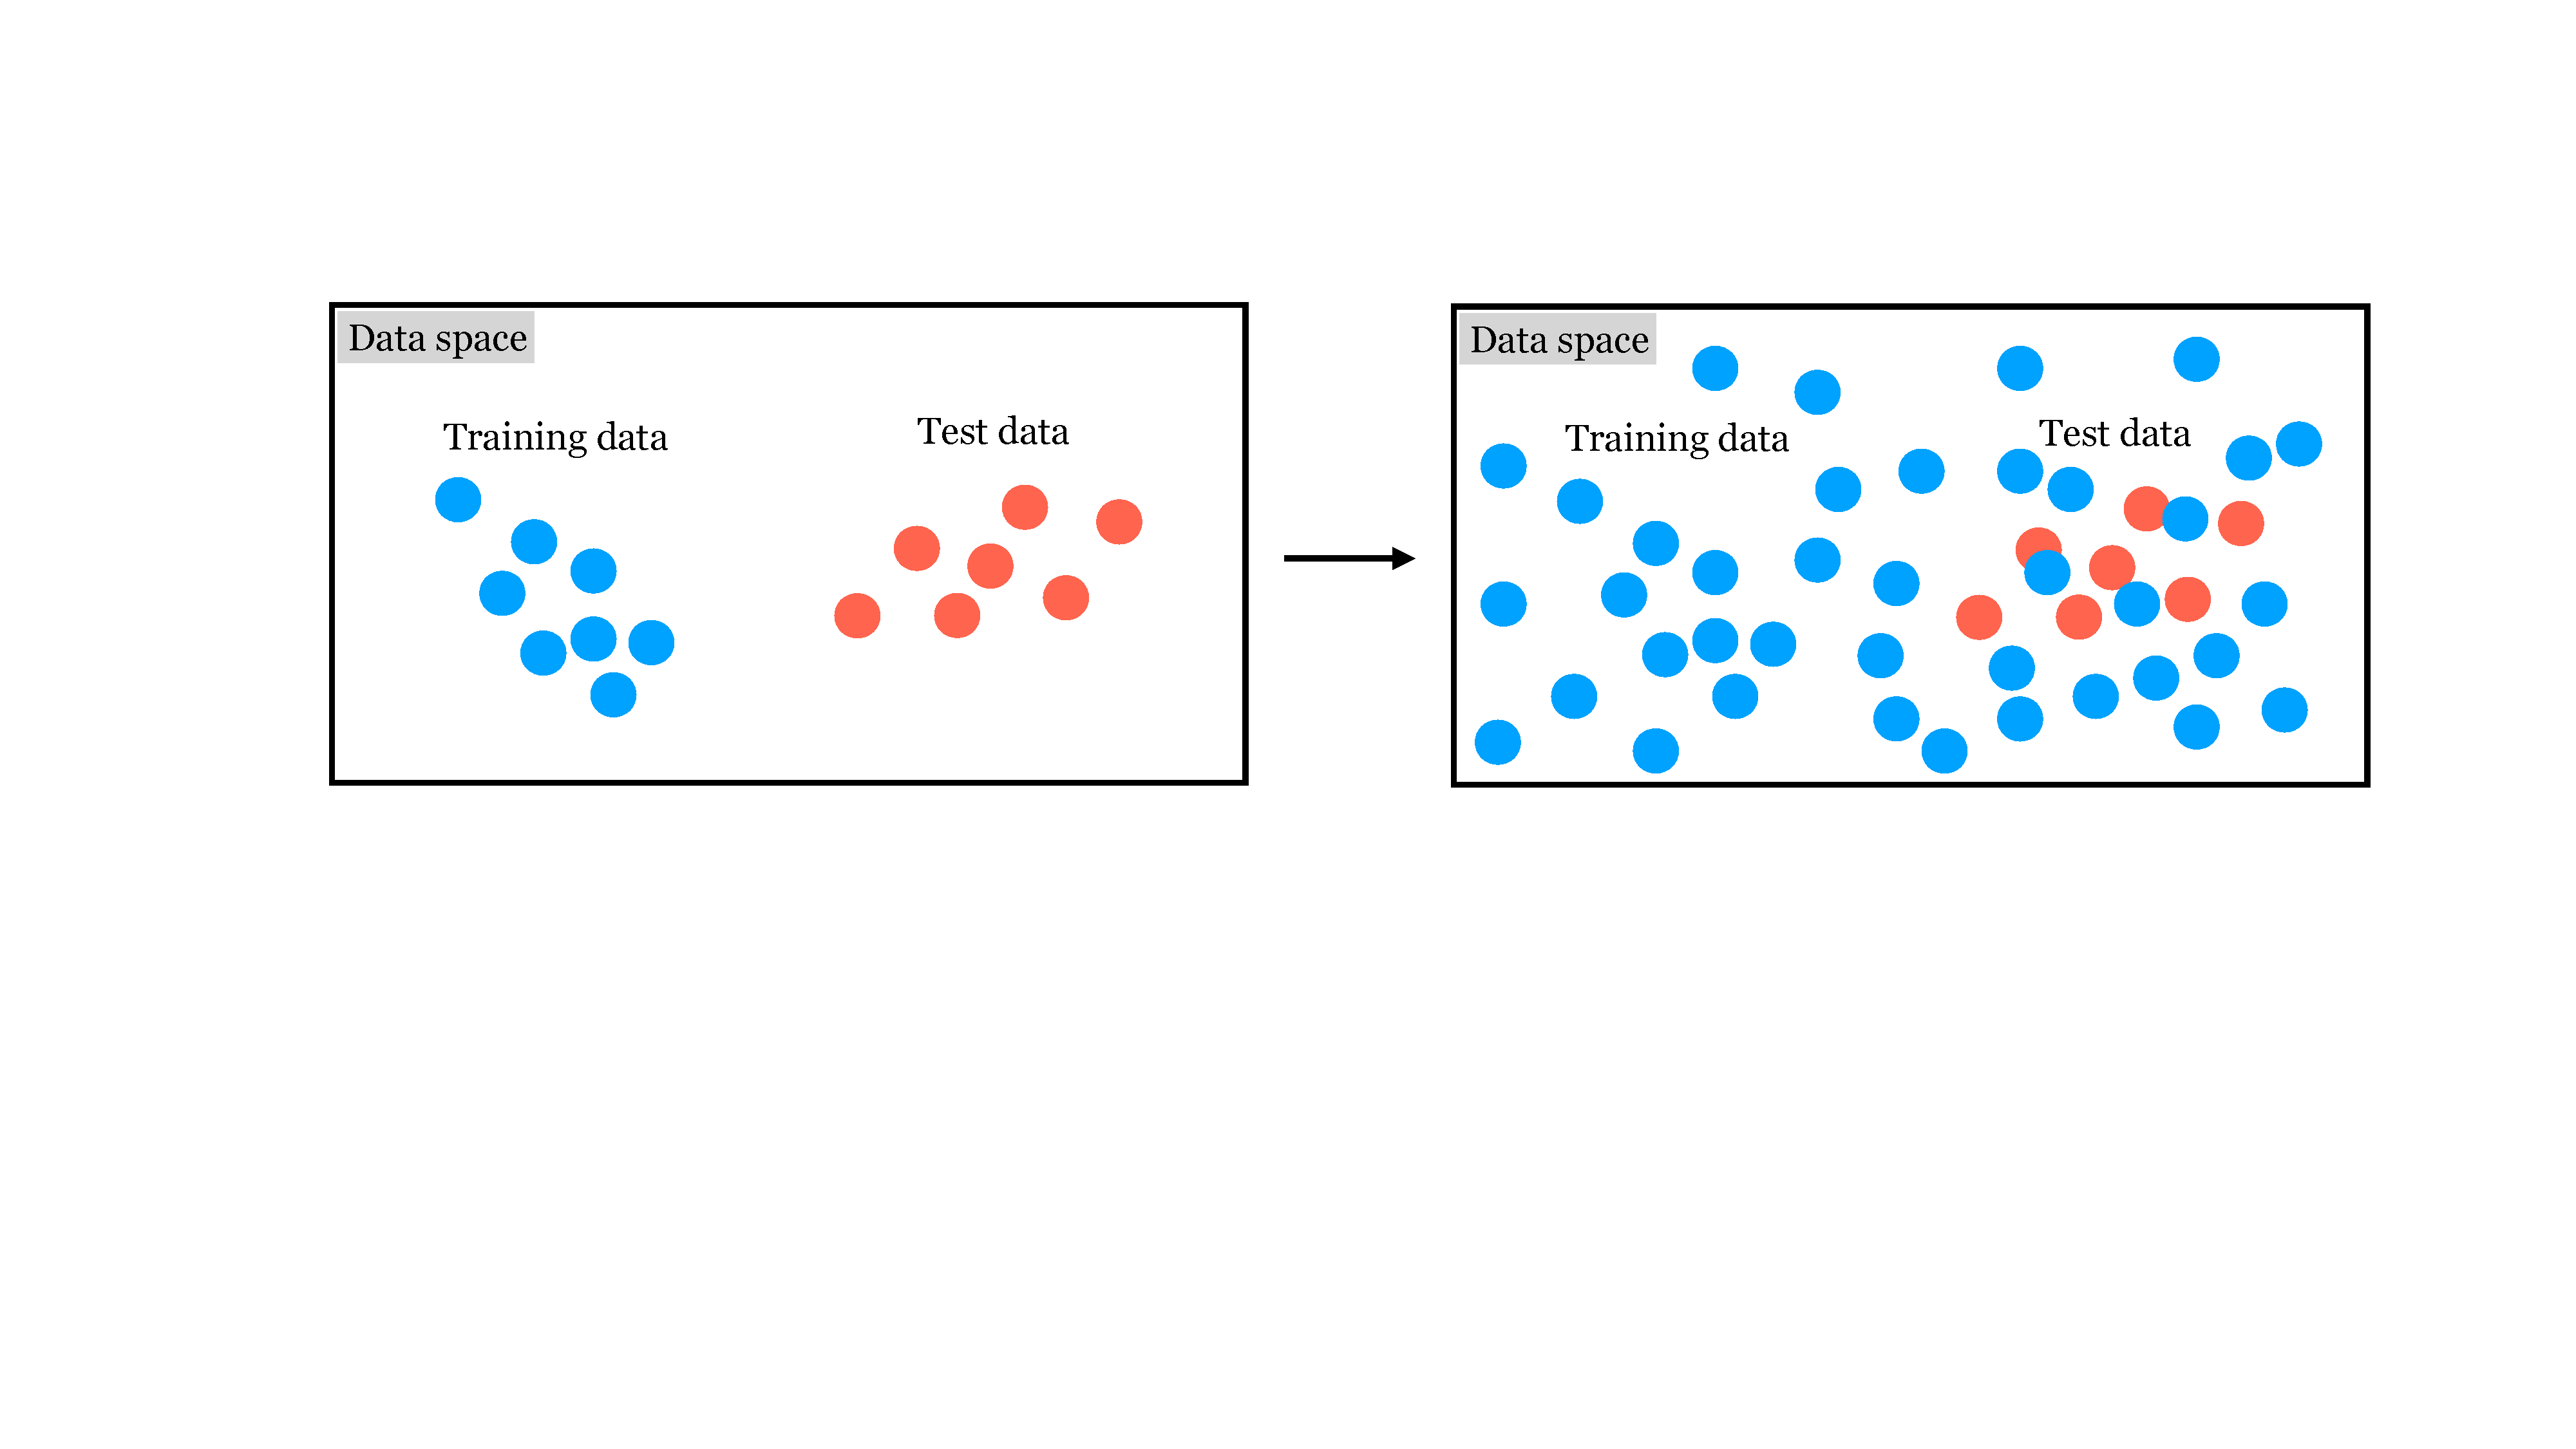
\includegraphics[width=1.0\linewidth]{./figures/data_augmentation/data_aug_scatter.pdf}
%     }
%     \caption{Data augmentation broadens the training data distribution so that it might better cover the test cases.}
%     \label{fig:data_augmentation:data_aug_scatter}
% \end{figure}
\begin{figure}[h]
    \centerline{
    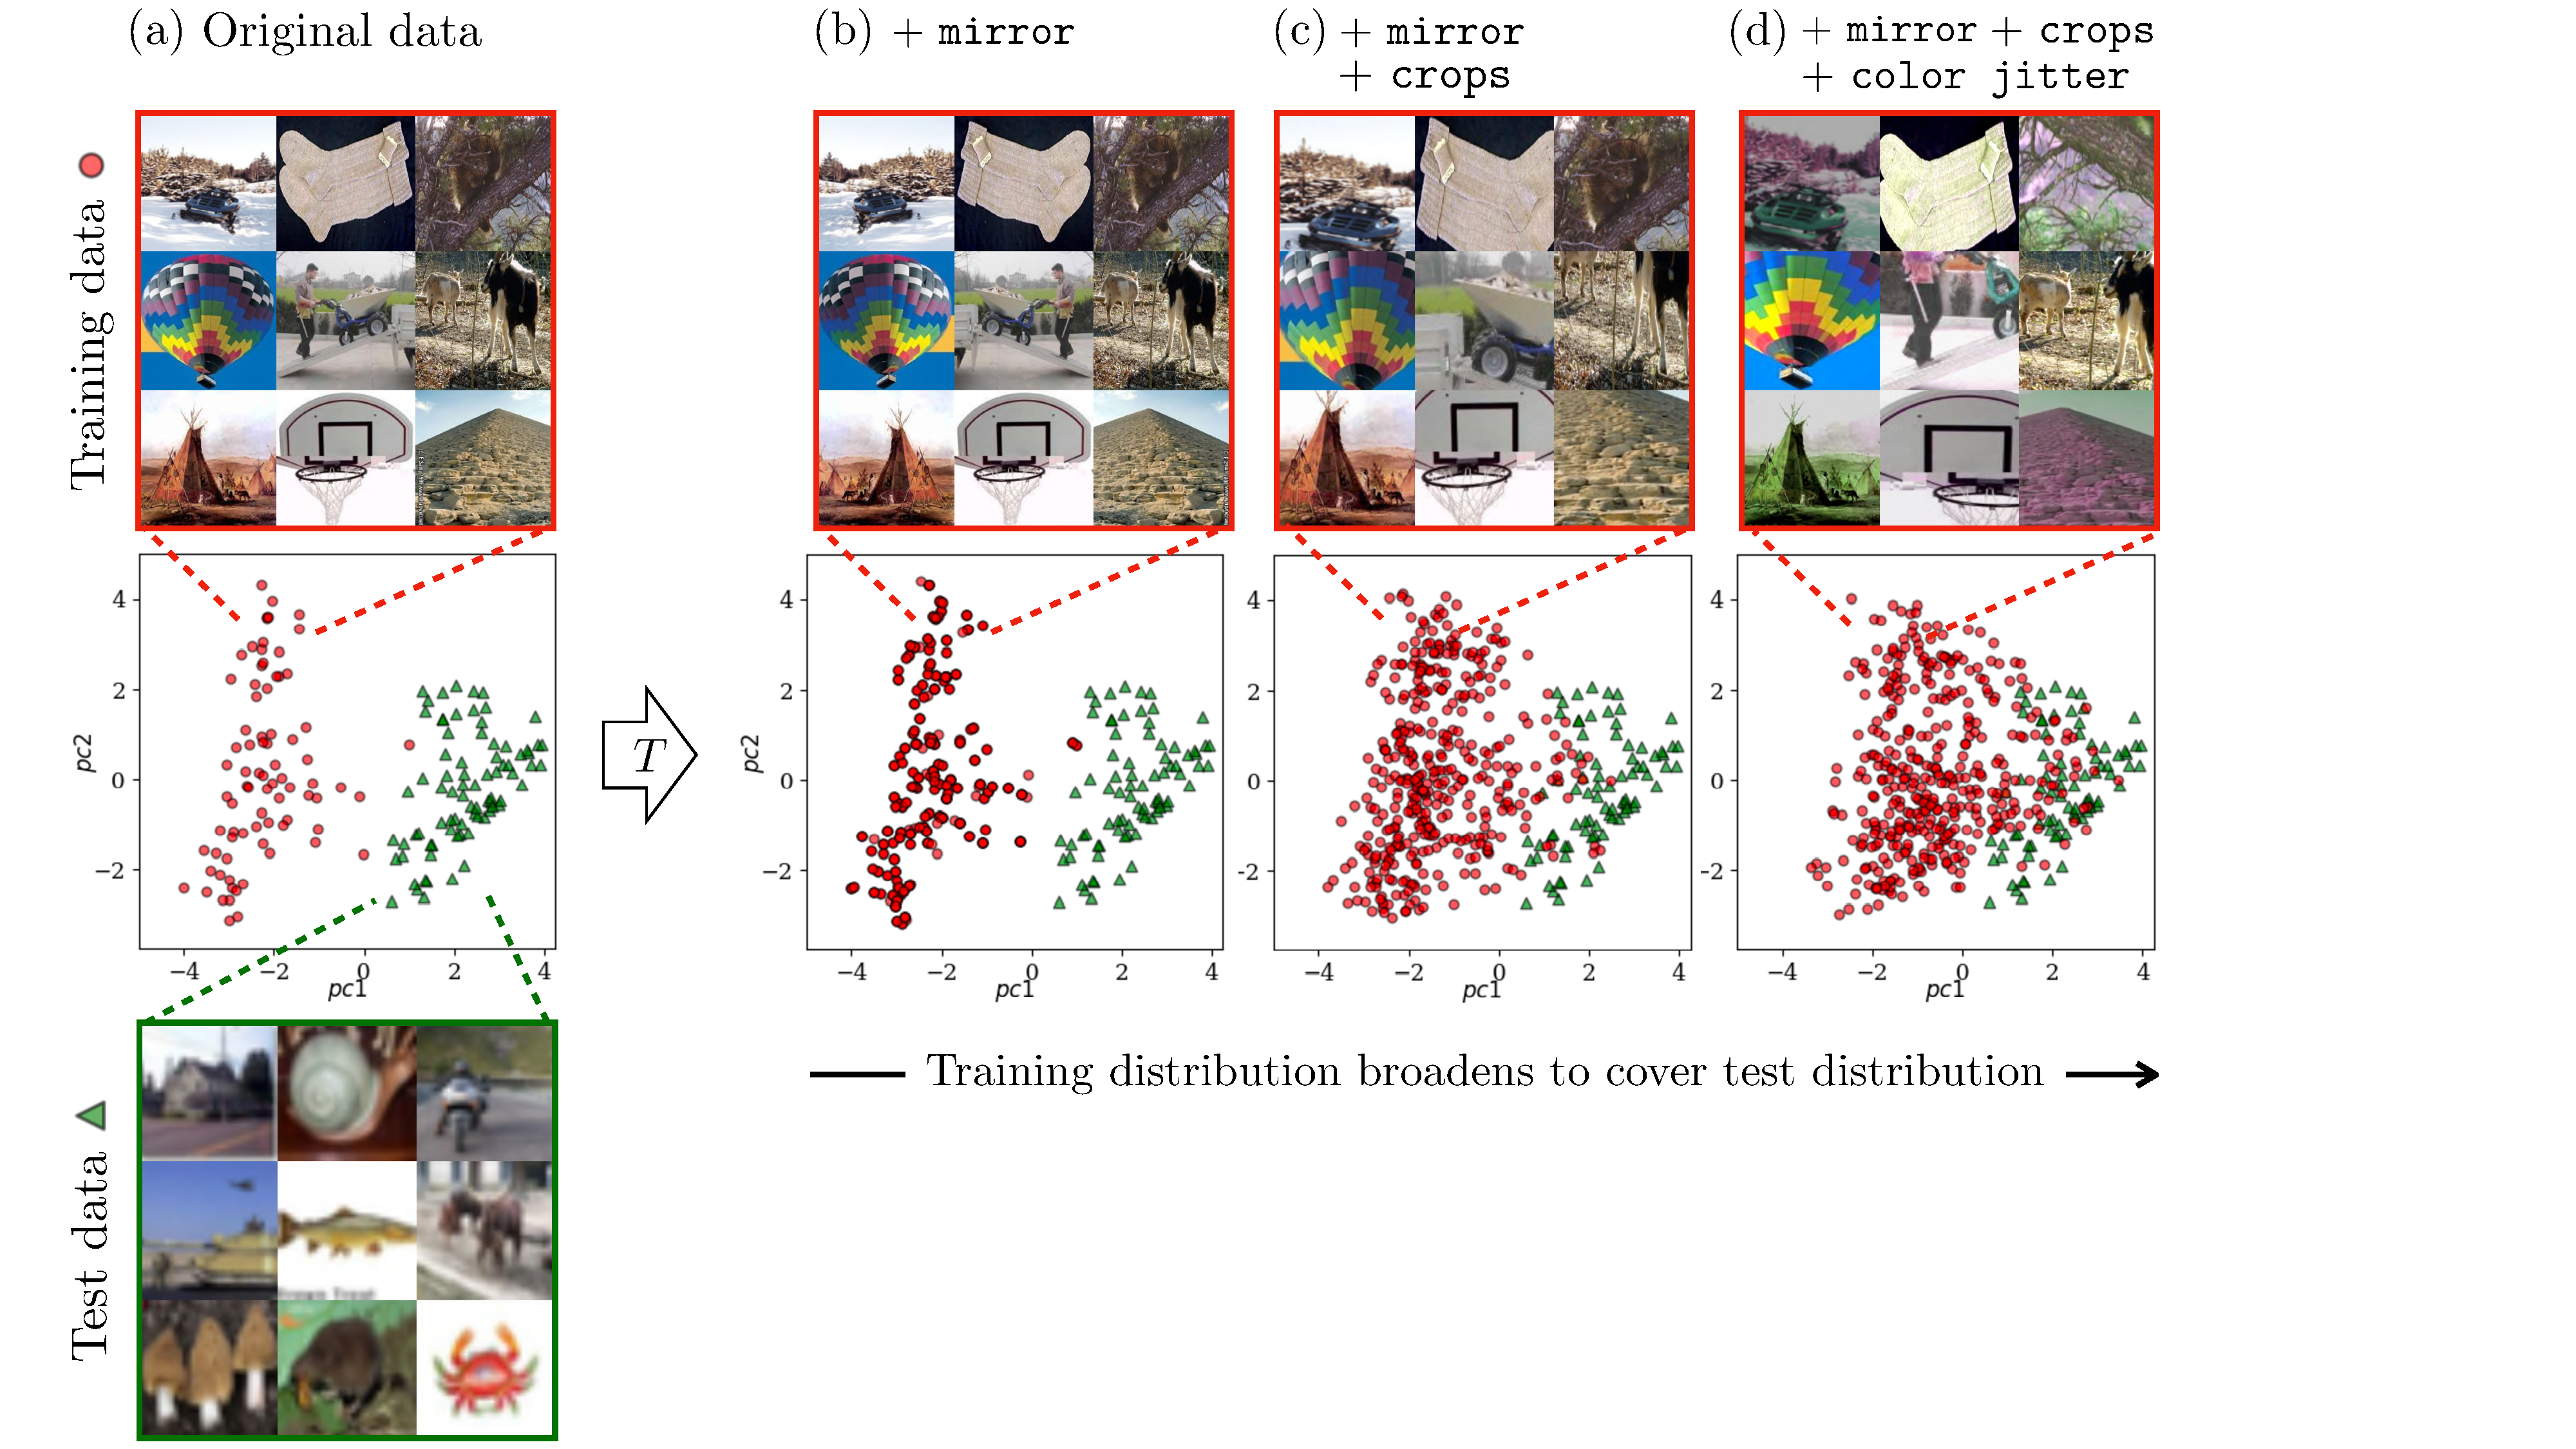
\includegraphics[width=1.0\linewidth]{./figures/data_augmentation/data_aug_real_example.pdf}
    }
    \caption{Data augmentation broadens the training distribution so that it might better cover the test cases. (a) Training data are from Caltech256~\cite{griffin2007caltech} and test data are from CIFAR100~\cite{cifar100}. The scatter plots show these data in a 2D feature space [the first two principle components (pcs) of CLIP~\cite{radford2021learning}]. (b) Training data after \texttt{mirror} augmentations (random horizontal flips). (c) The same plus \texttt{crops} (crop then rescale to the original size). (d) The same plus \texttt{color jitter} (random shifts in color and contrast).}
    \label{fig:data_augmentation:data_aug_real_example}
\end{figure}

\subsection{Learned Data Augmentation}
\index{Data augmentation!Learned}
Simple transformations like mirror flipping or cropping can be very effective while also being easy to implement by hand. After learning, the model will be invariant (or sometimes equivariant, if the $\mathbf{y}$ values are transformed too) with respect to these transformations. But these are just a few of all possible transformations that we might want to be invariant to. Imagine if we are building a pedestrian detector. Then we would probably like it to be invariant to pose variation in the pedestrian. This can be achieved by augmenting our data with random pose variations. But to do so may be very hard to code by hand. Instead we can use learning algorithms to \textit{learn} how to augment our data and achieve the invariances we would like.

One way to do this is to use generative models. Latent variable generative models like generative adversarial networks (GANs) or variational autoencoders (VAEs) are especially suitable, because the latent variables can be used to control different factors of variation in the generated data (see \chap{\ref{chapter:generative_modeling_and_representation_learning}}). Given a datapoint $\mathbf{x}$, an encoder $f_{\phi}: \mathcal{X} \rightarrow \mathcal{Z}$, and a generator $g_{\theta}: \mathcal{Z} \rightarrow \mathcal{X}$, we can create an augmented copy of $\mathbf{x}$ as, 
\begin{align}
    \mathbf{x} = g_{\theta}(f_{\psi}(\mathbf{x})+\mathbf{w}) \quad\quad \triangleleft \quad\text{generative data augmentation via latent manipulation}
\end{align}
\index{Data augmentation!Generative}
where $\mathbf{w}$ is a small perturbation to the latent variable $\mathbf{z}$. 
\marginnote{GANs do not necessarily come with encoders $f_{\psi}$, but for applications that need one, like we have here, you can simply train an encoder via supervised learning on pairs $\{g_{\theta}(\mathbf{z}), \mathbf{z}\}$, solving $\argmin_{\psi} \mathbb{E}_z [\mathcal{L}(f_{\psi}(g_{\theta}(\mathbf{z})), \mathbf{z})]$. See \cite{donahue2016adversarial} for discussion of this method and more advanced techniques.}[-3.6cm]
If we do this for a variety of settings of $\mathbf{w}$, then we will get a set of output images that are all slight variations of one another, just like we saw previously in \fig{\ref{fig:generative_modeling_and_representation_learning:biggan_latent_walk}}. One simple approach is to just use Gaussian perturbations in latent space, that is, $\mathbf{w} \sim \mathcal{N}(0,\sigma^2)$ for some perturbation scale given by $\sigma$. 
%, which may be small perturbations or axis-aligned so that they capture the independent factors of variation discovered by the model. 
\Algref{\ref{alg:data_augmentation:generative_data_augmentation}} formalizes this approach (see \cite{chai2021ensembling} for a representative work that roughly follows this recipe, or \cite{azizi2023synthetic} for an alternative approach to generative data augmentation).
\begin{algorithm}[h]
\SetAlgoVlined
\DontPrintSemicolon
%\marginnote{{\bf Algorithm \ref{alg:data_augmentation:generative_data_augmentation}}: Using a generative model to augment a dataset.}
\caption{{\bf Algorithm \ref{alg:data_augmentation:generative_data_augmentation}}: Generative data augmentation (\texttt{genaug}). }
\fakealgorithmcaption{}
\label{alg:data_augmentation:generative_data_augmentation}
{\bf Input:} Generative model $g_{\theta}: \mathcal{Z} \rightarrow \mathcal{X}$ and its (approximate) inverse $f_{\psi}: \mathcal{X} \rightarrow \mathcal{Z}$, perturbation scale parameter $\sigma$, Dataset $X \triangleq \{\mathbf{x}^{(i)},\mathbf{y}^{(i)}\}_{i=1}^N$, hyperparameter $k$\;
{\bf Output:} Augmented dataset $\tilde{X} \triangleq \{\tilde{\mathbf{x}}^{(i)}, \tilde{\mathbf{y}}^{(i)}\}_{i=1}^{kN}$\;
\For{\upshape $i = 1, \dots, N$} {
    \For{\upshape $j = 1, \dots, k$} {
        $\mathbf{z}^{(i)} = f_{\psi}(\mathbf{x}^{(i)})$ \;
        $\mathbf{w}_j \sim \mathcal{N}(0,\sigma^2)$ \;
        $\tilde{X} \leftarrow \{g_{\theta}(\mathbf{z}^{(i)}+\mathbf{w}_j), \mathbf{y}^{(i)}\}$ \;
    }
}
\end{algorithm}

%Where $\texttt{randaug()}$ is a task-specific function that applies a perturbation in $z$-space (a simple choice might be that $\texttt{randaug}$ just returns a Gaussian vector, i.e., $\mathbf{w}_j \sim \mathcal{N}(0,\sigma)$ for some perturbation scale given by $\sigma$).


% \begin{figure}[h]
There are some subtleties when working with learned data augmentation. You might be tempted to train $g_{\theta}$ on the same dataset you are trying to augment, that is, train $g_{\theta}$ on $X$, then use $g_{\theta}$ to augment $X$. This can have interesting regularizing effects, but it introduces an uncomfortable circularity, which can be understood as follows. We want to create augmented data for training some function $f$. Let the learner for $f$ be denoted as the function $L$, which is a mapping from input data to output learned function $f$. \marginnote{It can be confusing to think of a learning \textit{algorithm} as a \textit{function}, but that's what it is; as we pointed out in \chap{\ref{chapter:intro_to_learning}}, a learner is a function that outputs a function.}[-0.4cm]
Without data augmentation we have $f = L(X)$, and with data augmentation we have $f = L(\tilde{X})$. But now, when $g_{\theta}$ is trained on $X$, then $\tilde{X}$ is just a function of $X$; in particular, if we use \algref{\ref{alg:data_augmentation:generative_data_augmentation}}, it is $\tilde{X} = \texttt{genaug}(X)$. So, we can define a new learner $\tilde{L} = L \circ \texttt{genaug}$ where we have $f = \tilde{L}(X) = L(\texttt{genaug}(X)) = L(\tilde{X})$. This demonstrates that there exists a learning algorithm, $\tilde{L}$, that uses unaugmented data and is just as good as our learning algorithm that used augmented data.

A clearer gain can be achieved by using a $g_{\theta}$ pretrained on external data. For example, if we have a general purpose image generative model, trained on millions of images (such as \cite{ramesh2022hierarchical} or \cite{rombach2022high}), then we can use it to augment a small dataset for a new specific task we come across. %See XX and YY for representative explorations of this approach.


% \begin{tikzpicture}
% \begin{axis}[view={0}{90}, xmin=-1, xmax=1, ymin=-1, ymax=1, 
% name=plot1,
% width=0.4\linewidth,
% align=center,
% title={Without data augmentation},
% scatter/classes={%
%     train={mark=*, draw=blue},%
%     test={mark=*, draw=red}}]
% %
% \addplot[scatter,only marks]%
% table[meta=label] {
% x y label
% 0.1 0.3 train
% 0.3 0.15 train
% 0.4 0.5 train
% -0.1 0.71 train
% -0.4 0.31 train
% -0.7 0.54 train
% %
% -0.5 -0.68 test
% -0.2 -0.23 test
% -0.12 -0.67 test
% 0.07 -0.47 test
% 0.42 -0.28 test
% 0.7 -0.54 test
%     };
% \end{axis}
% %\end{tikzpicture}
% %\begin{tikzpicture}
% %
% \draw[thick] [flow_arrow] (4.5,1.6) -- (5.5,1.6);
% %
% \begin{axis}[view={0}{90}, xmin=-1, xmax=1, ymin=-1, ymax=1, 
% width=0.4\linewidth,
% at=(plot1.right of south east), anchor=left of south west,
% xshift=1cm,
% align=center,
% title={With data augmentation},
% scatter/classes={%
%     train={mark=*, draw=blue},%
%     test={mark=*, draw=red}}]
% %
% \addplot[scatter,only marks]%
% table[meta=label] {
% x y label
% 0.1 0.3 train
% 0.3 0.15 train
% 0.4 0.5 train
% -0.1 0.71 train
% -0.4 0.31 train
% -0.7 0.54 train
% %
% -0.5 -0.68 test
% -0.2 -0.23 test
% -0.12 -0.67 test
% 0.07 -0.47 test
% 0.42 -0.28 test
% 0.7 -0.54 test
%     };
% \end{axis}
% \end{tikzpicture}
% \end{figure}

%Diagram of the equivariant mapping?


\section{Adversarial Training}

With data augmentation, the learning problem looks like this:
\begin{align}
    \argmin_f \mathbb{E}_{\mathbf{x},\mathbf{y}} [\mathbb{E}_{\theta \sim p_{\theta}}[\mathcal{L}(f(T(\mathbf{x};\theta)),\mathbf{y})]]
\end{align}
Here we are applying random transformations to the data, and we want our learner to do well in expectation over these random transformations. Instead of doing random transformations, we could instead consider augmenting with \textit{worst case} transformations, applying those transformations that incur the highest loss possible for a given training example:
\begin{align}
    \argmin_f \mathbb{E}_{\mathbf{x},\mathbf{y}} [\max_{\theta \in \Theta}[\mathcal{L}(f(T(\mathbf{x};\theta)),\mathbf{y})]] \label{eqn:data_augmentation:adversarial_training}
\end{align}
This idea is known as \index{Adversarial training}{\bf adversarial training}. One of its effects is that it can increase the robustness of the learned function $f$ to perturbations that may occur at test time (like those we saw in the previous chapter).

In the context of adversarial robustness, one form of \eqn{\ref{eqn:data_augmentation:adversarial_training}} is to set $T$ to be an epsilon-ball attack, that is, $T(\mathbf{x}) = \mathbf{x}+\mathbf{\epsilon}$:
\begin{align}
    \argmin_f \mathbb{E}_{\mathbf{x},\mathbf{y}} [\max_{\mathbf{\epsilon} \, s.t. \norm{\mathbf{\epsilon}} < r}[\mathcal{L}(f(\mathbf{x}+\mathbf{\epsilon}),\mathbf{y})]] \label{eqn:data_augmentation:eps_robust_training}
\end{align}
This can increase robustness against the kinds of epsilon-ball attacks we saw in the previous chapter.

Adversarial training has many other uses as well, beyond the scope of the current chapter: it is used for training generative adversarial networks (\chap{\ref{chapter:generative_models}}), for training agents to explore in reinforcement learning~\cite{pathak2017curiosity}, and for training agents that compete against other agents~\cite{silver2016mastering}. This general approach is also known as \textbf{robust optimization} in the optimization literature.

\section{Toward General-Purpose Vision Models}

The lesson from this chapter is that if you train on more and more data, you can achieve better coverage over all the test cases you might encounter. This raises a natural question: Rather than inventing new augmentation and robustness methods, why not just collect ever more data? This approach is becoming increasingly dominant, and a major focus of current efforts is on just scaling the training data size and diversity. 

\subsection{Multitask training}
\index{Multitask training}
Because we have finite data for any given task, it can help to share data between tasks. Suppose we have two tasks, $A$ and $B$. How can we borrow data from task $B$ to increase the data available for task $A$? In line with the theme of this chapter, one approach is to not just broaden the \textit{data} but to also broaden the \textit{task}. The idea is to define a new task, $AB$, for which tasks $A$ and $B$ are special cases. Then we can train $AB$ on both the data for task $A$ and for task $B$. An example of a metatask like $AB$ is data imputation (see \chap{\ref{chapter:generative_modeling_and_representation_learning}}). One example of data imputation is to predict missing color channels; this is the colorization problem, call this task $A$. Another data imputation problem is predicting a chunk of pixels masked out of the image; this is the inpainting problem, which we can call task $B$. We can train a joint colorization–inpainting model if we simply set up both as data imputation and train a general data imputation model. This model can be trained on both colorization training data and inpainting training data.\marginnote{Data imputation is an incredibly general framework. Can you think of other vision problems that can be formulated as data imputation? Or, here is a harder question: Can you think of any vision problems that cannot be formulated this way?}[-3.4cm]

In the next chapter, we will see several more examples of how to make use of data from task $B$ for task $A$.


\section{Concluding Remarks}

A grand challenge of computer vision is to make algorithms that work in \textit{general}, no matter the setting in which you deploy them. For example, we would like object detectors that will recognize a cat on the internet, a cat in your house, a cat on Mars, an upside down cat, and so on. One of the simplest ways to achieve this is to train for generality: train your system on as much data, as diverse data, and as many tasks as possible. This approach is, perhaps, the main reason we now have computer vision systems that really work in practice, whereas a decade ago we didn't.

%There are two ways to make a vision system work in a broader range of contexts and solve a broader range of problems: either train for generality or design algorithms that adapt quickly to new problems. The former was the topic of this chapter and it has been the main story behind the success of vision systems in the deep learning era.